\documentclass[10pt]{beamer}

\usetheme{metropolis}
\usepackage{appendixnumberbeamer}

\usepackage{booktabs}
\usepackage[scale=2]{ccicons}

\usepackage{pgfplots}
\usepgfplotslibrary{dateplot}

\usepackage{xspace}
\newcommand{\themename}{\textbf{\textsc{metropolis}}\xspace}

\usepackage{caption}
\captionsetup[figure]{labelformat=empty}% redefines the caption setup of the figures environment in the beamer class.


\title{Git}
\subtitle{A short introduction}
\date{\today}
\author{Tristan Igelbrink}
\institute{Hochschule Osnabrück}
% \titlegraphic{\hfill\includegraphics[height=1.5cm]{logo.pdf}}

\begin{document}

\maketitle

%\begin{frame}{Table of contents}
%  \setbeamertemplate{section in toc}[sections numbered]
%  \tableofcontents[hideallsubsections]
%\end{frame}

\section{What means version control?}

\begin{frame}[fragile]{What means version control?}
    \begin{alertblock}{Management for developing things in a team}
     \begin{itemize}
       \item Simultaneously working on the same files
       \item Backup files
       \item Generate a modification history
       \item Jump in time
      \end{itemize}
    \end{alertblock}
    \begin{figure}[t]
       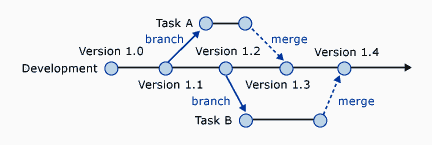
\includegraphics[scale=0.6]{version_control_alpha.png} 
    \end{figure}
\end{frame}

\begin{frame}{What means version control?}
    	\begin{figure}[t]
      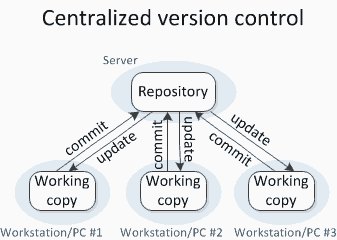
\includegraphics[width=0.45\textwidth]{centralized_version_control.png}
    \end{figure}
    \begin{figure}[t]
      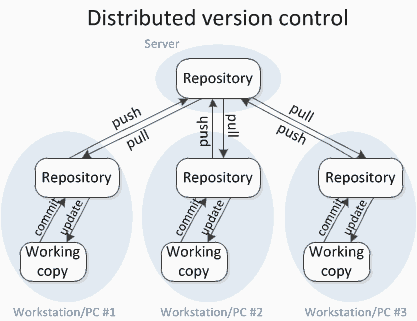
\includegraphics[width=0.45\textwidth]{dist_version_control.png}
    \end{figure}
\end{frame}

\section{Git}

\begin{frame}{Git}
    	\begin{figure}[t]
      
\includegraphics[width=0.28\textwidth]{git_logo.png}
    \end{figure}
    \begin{alertblock}{Git}
     \begin{itemize}
       \item Open-source version control system
       \item Initially designed and developed in 2005 by Linus Torvalds for the develoment of the Linux Kernel
       \item Distributed and highly efficient
       \item Widely used for Open-source software development 
      \end{itemize}
    \end{alertblock}
\end{frame}

\begin{frame}{Git}
   \begin{alertblock}{Git workflow}
    	\begin{figure}[t]
      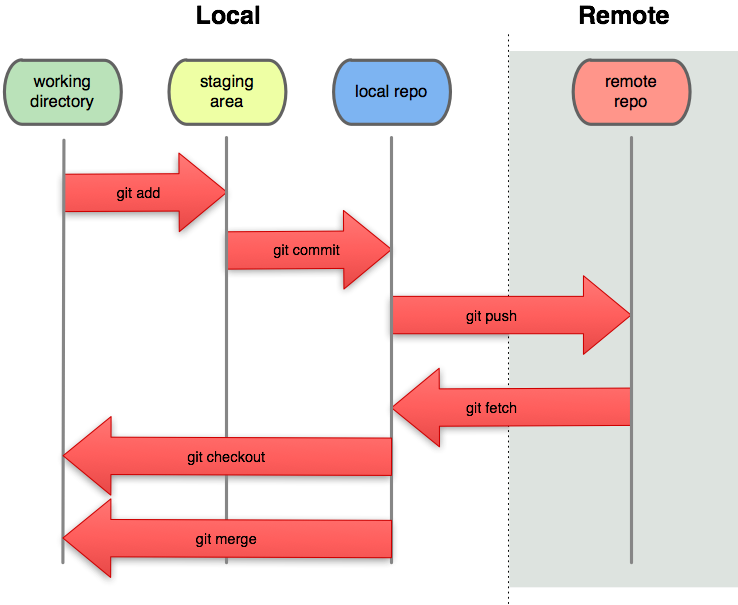
\includegraphics[width=0.75\textwidth]{git_workflow.png}
    \end{figure}
   \end{alertblock}
\end{frame}

\begin{frame}{Git}
   \begin{alertblock}{GUI Gitg}
    	\begin{figure}[t]
      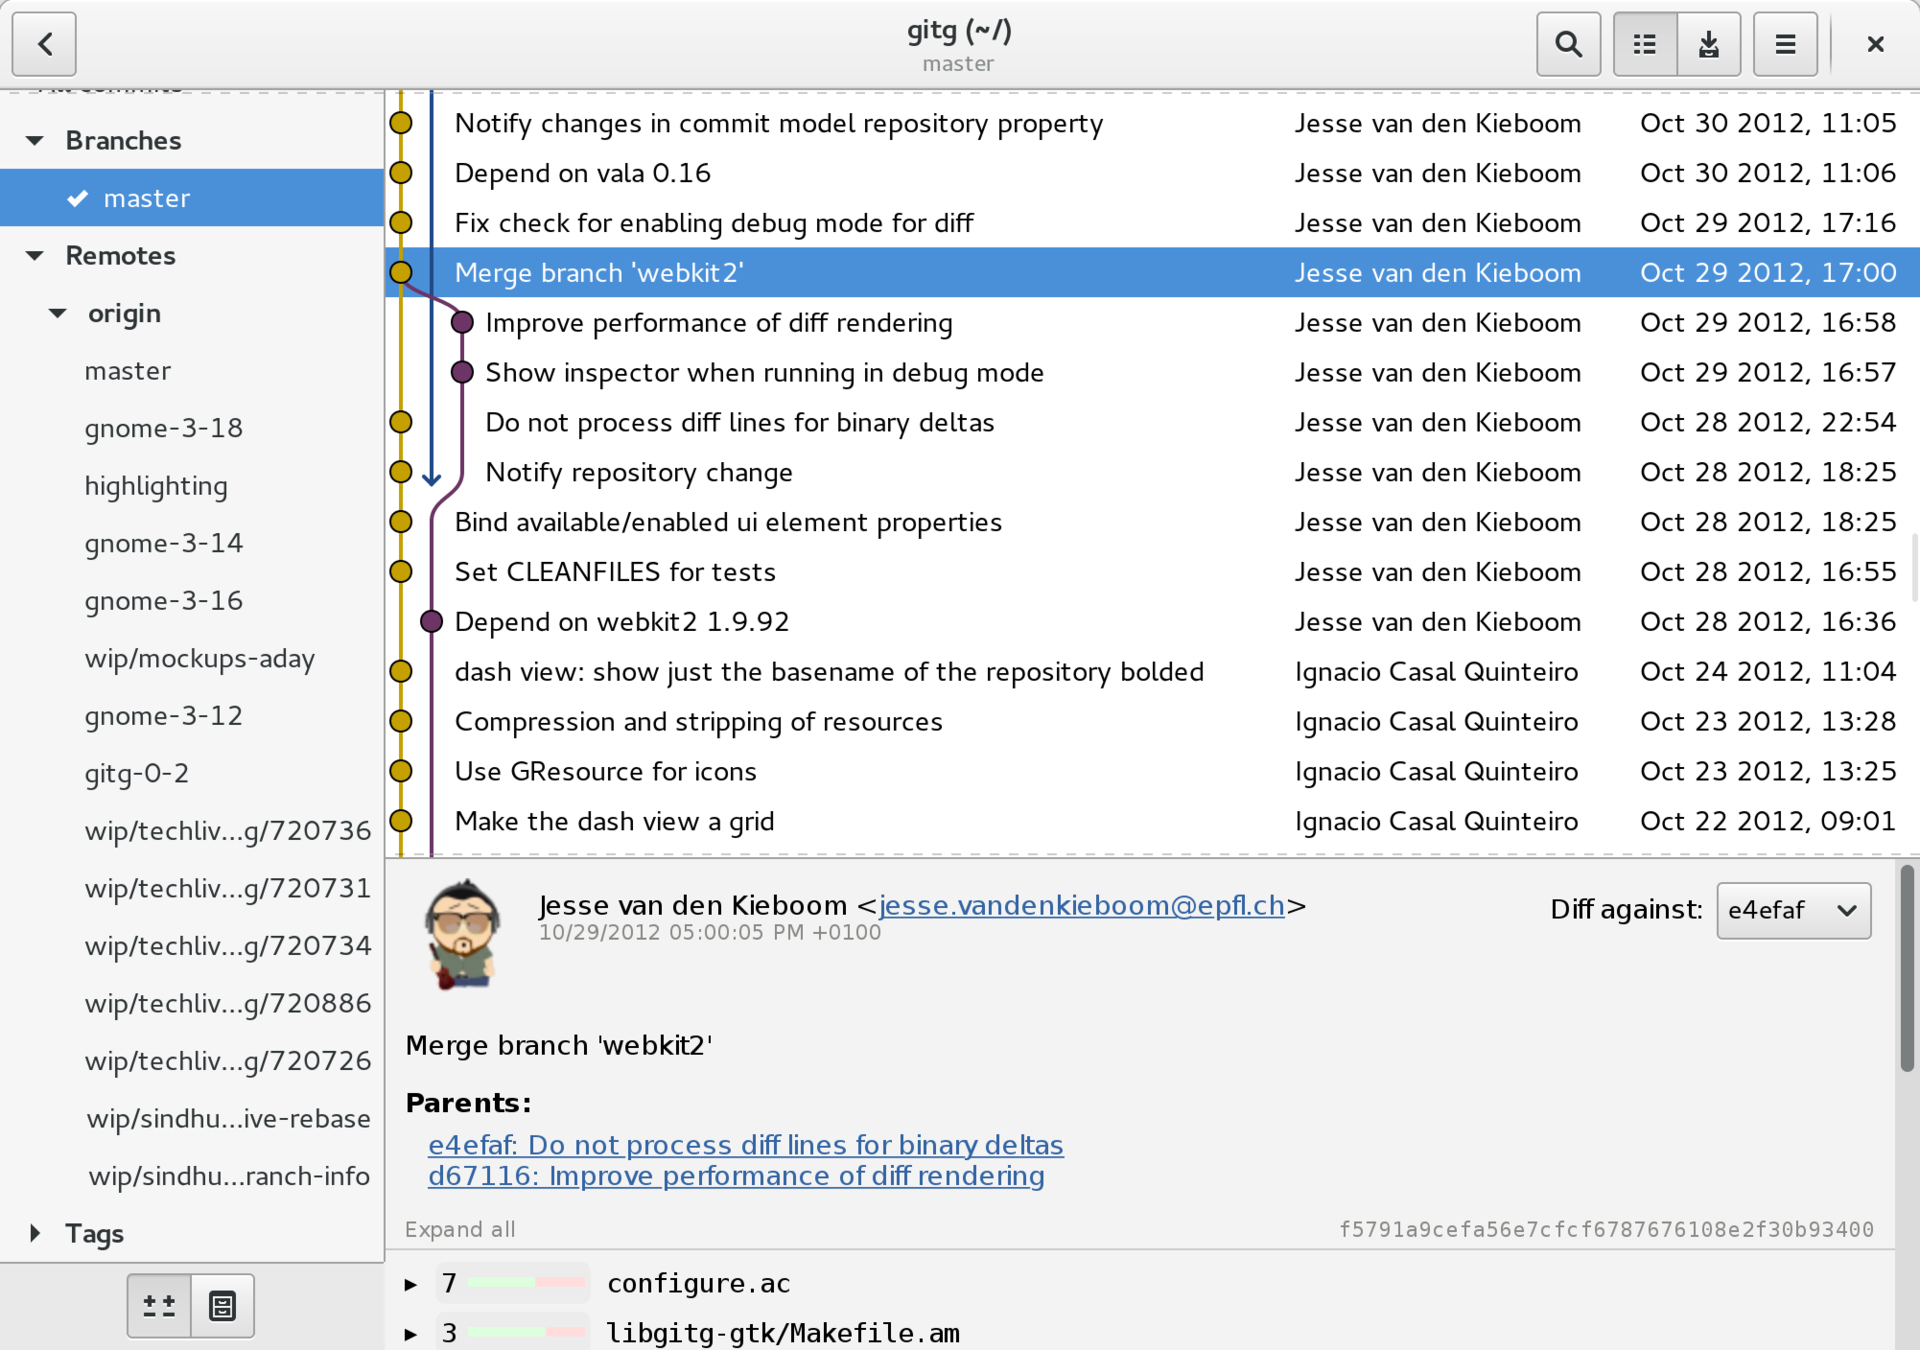
\includegraphics[width=0.8\textwidth]{gitg_gui.png}
    \end{figure}
   \end{alertblock}
\end{frame}



\begin{frame}[standout]
  Questions?
\end{frame}

\end{document}
